\documentclass{article}
\usepackage{ifthen}
\usepackage{amssymb}
\usepackage{multicol}
\usepackage{graphicx}
\usepackage[absolute]{textpos}

\usepackage[noload]{qtree}
%\usepackage{xspace,rotating,calligra,dsfont,ifthen}
\usepackage{xspace,rotating,dsfont,ifthen}
\usepackage[spanish,activeacute]{babel}
\usepackage[utf8]{inputenc}
\usepackage{pgfpages}
\usepackage{pgf,pgfarrows,pgfnodes,pgfautomata,pgfheaps,xspace,dsfont}
\usepackage{listings}
\usepackage{multicol}


\makeatletter

\@ifclassloaded{beamer}{%
  \newcommand{\tocarEspacios}{%
    \addtolength{\leftskip}{4em}%
    \addtolength{\parindent}{-3em}%
  }%
}
{%
  \usepackage[top=1cm,bottom=2cm,left=1cm,right=1cm]{geometry}%
  \usepackage{color}%
  \newcommand{\tocarEspacios}{%
    \addtolength{\leftskip}{5em}%
    \addtolength{\parindent}{-3em}%
  }%
}

\newcommand{\encabezadoDeProc}[4]{%
  % Ponemos la palabrita problema en tt
%  \noindent%
  {\normalfont\bfseries\ttfamily proc}%
  % Ponemos el nombre del problema
  \ %
  {\normalfont\ttfamily #2}%
  \
  % Ponemos los parametros
  (#3)%
  \ifthenelse{\equal{#4}{}}{}{%
  \ =\ %
  % Ponemos el nombre del resultado
  {\normalfont\ttfamily #1}%
  % Por ultimo, va el tipo del resultado
  \ : #4}
}

\newcommand{\encabezadoDeTipo}[2]{%
  % Ponemos la palabrita tipo en tt
  {\normalfont\bfseries\ttfamily tipo}%
  % Ponemos el nombre del tipo
  \ %
  {\normalfont\ttfamily #2}%
  \ifthenelse{\equal{#1}{}}{}{$\langle$#1$\rangle$}
}

% Primero definiciones de cosas al estilo title, author, date

\def\materia#1{\gdef\@materia{#1}}
\def\@materia{No especifi\'o la materia}
\def\lamateria{\@materia}

\def\cuatrimestre#1{\gdef\@cuatrimestre{#1}}
\def\@cuatrimestre{No especifi\'o el cuatrimestre}
\def\elcuatrimestre{\@cuatrimestre}

\def\anio#1{\gdef\@anio{#1}}
\def\@anio{No especifi\'o el anio}
\def\elanio{\@anio}

\def\fecha#1{\gdef\@fecha{#1}}
\def\@fecha{\today}
\def\lafecha{\@fecha}

\def\nombre#1{\gdef\@nombre{#1}}
\def\@nombre{No especific'o el nombre}
\def\elnombre{\@nombre}

\def\practicas#1{\gdef\@practica{#1}}
\def\@practica{No especifi\'o el n\'umero de pr\'actica}
\def\lapractica{\@practica}


% Esta macro convierte el numero de cuatrimestre a palabras
\newcommand{\cuatrimestreLindo}{
  \ifthenelse{\equal{\elcuatrimestre}{1}}
  {Primer cuatrimestre}
  {\ifthenelse{\equal{\elcuatrimestre}{2}}
  {Segundo cuatrimestre}
  {Verano}}
}


\newcommand{\depto}{{UBA -- Facultad de Ciencias Exactas y Naturales --
      Departamento de Computaci\'on}}

\newcommand{\titulopractica}{
  \centerline{\depto}
  \vspace{1ex}
  \centerline{{\Large\lamateria}}
  \vspace{0.5ex}
  \centerline{\cuatrimestreLindo de \elanio}
  \vspace{2ex}
  \centerline{{\huge Pr\'actica \lapractica -- \elnombre}}
  \vspace{5ex}
  \arreglarincisos
  \newcounter{ejercicio}
  \newenvironment{ejercicio}{\stepcounter{ejercicio}\textbf{Ejercicio
      \theejercicio}%
    \renewcommand\@currentlabel{\theejercicio}%
  }{\vspace{0.2cm}}
}


\newcommand{\titulotp}{
  \centerline{\depto}
  \vspace{1ex}
  \centerline{{\Large\lamateria}}
  \vspace{0.5ex}
  \centerline{\cuatrimestreLindo de \elanio}
  \vspace{0.5ex}
  \centerline{\lafecha}
  \vspace{2ex}
  \centerline{{\huge\elnombre}}
  \vspace{5ex}
}


%practicas
\newcommand{\practica}[2]{%
    \title{Pr\'actica #1 \\ #2}
    \author{Algoritmos y Estructuras de Datos I}
    \date{Primer Cuatrimestre 2018}

    \maketitlepractica{#1}{#2}
}

\newcommand \maketitlepractica[2] {%
\begin{center}
\begin{tabular}{r cr}
 \begin{tabular}{c}
{\large\bf\textsf{\ Algoritmos y Estructuras de Datos I\ }}\\
Primer Cuatrimestre 2018\\
\title{\normalsize Gu\'ia Pr\'actica #1 \\ \textbf{#2}}\\
\@title
\end{tabular} &
\begin{tabular}{@{} p{1.6cm} @{}}
\includegraphics[width=1.6cm]{logodpt.jpg}
\end{tabular} &
\begin{tabular}{l @{}}
 \emph{Departamento de Computaci\'on} \\
 \emph{Facultad de Ciencias Exactas y Naturales} \\
 \emph{Universidad de Buenos Aires} \\
\end{tabular}
\end{tabular}
\end{center}

\bigskip
}


% Simbolos varios

\newcommand{\ent}{\ensuremath{\mathds{Z}}}
\newcommand{\float}{\ensuremath{\mathds{R}}}
\newcommand{\bool}{\ensuremath{\mathsf{Bool}}}
\newcommand{\True}{\ensuremath{\mathrm{true}}}
\newcommand{\False}{\ensuremath{\mathrm{false}}}
\newcommand{\Then}{\ensuremath{\rightarrow}}
\newcommand{\Iff}{\ensuremath{\leftrightarrow}}
\newcommand{\implica}{\ensuremath{\longrightarrow}}
\newcommand{\IfThenElse}[3]{\ensuremath{\mathsf{if}\ #1\ \mathsf{then}\ #2\ \mathsf{else}\ #3\ \mathsf{fi}}}
\newcommand{\In}{\textsf{in }}
\newcommand{\Out}{\textsf{out }}
\newcommand{\Inout}{\textsf{inout }}
\newcommand{\yLuego}{\land _L}
\newcommand{\oLuego}{\lor _L}
\newcommand{\implicaLuego}{\implica _L}
\newcommand{\existe}[3]{\ensuremath{(\exists #1:\ent) \ #2 \leq #1 < #3 \ }}
\newcommand{\paraTodo}[3]{\ensuremath{(\forall #1:\ent) \ #2 \leq #1 < #3 \ }}

% Símbolo para marcar los ejercicios importantes (estrellita)
\newcommand\importante{\raisebox{0.5pt}{\ensuremath{\bigstar}}}


\newcommand{\rango}[2]{[#1\twodots#2]}
\newcommand{\comp}[2]{[\,#1\,|\,#2\,]}

\newcommand{\rangoac}[2]{(#1\twodots#2]}
\newcommand{\rangoca}[2]{[#1\twodots#2)}
\newcommand{\rangoaa}[2]{(#1\twodots#2)}

%ejercicios
\newtheorem{exercise}{Ejercicio}
\newenvironment{ejercicio}[1][]{\begin{exercise}#1\rm}{\end{exercise} \vspace{0.2cm}}
\newenvironment{items}{\begin{enumerate}[a)]}{\end{enumerate}}
\newenvironment{subitems}{\begin{enumerate}[i)]}{\end{enumerate}}
\newcommand{\sugerencia}[1]{\noindent \textbf{Sugerencia:} #1}

\lstnewenvironment{code}{
    \lstset{% general command to set parameter(s)
        language=C++, basicstyle=\small\ttfamily, keywordstyle=\slshape,
        emph=[1]{tipo,usa}, emphstyle={[1]\sffamily\bfseries},
        morekeywords={tint,forn,forsn},
        basewidth={0.47em,0.40em},
        columns=fixed, fontadjust, resetmargins, xrightmargin=5pt, xleftmargin=15pt,
        flexiblecolumns=false, tabsize=2, breaklines, breakatwhitespace=false, extendedchars=true,
        numbers=left, numberstyle=\tiny, stepnumber=1, numbersep=9pt,
        frame=l, framesep=3pt,
    }
   \csname lst@SetFirstLabel\endcsname}
  {\csname lst@SaveFirstLabel\endcsname}


%tipos basicos
\newcommand{\rea}{\ensuremath{\mathsf{Float}}}
\newcommand{\cha}{\ensuremath{\mathsf{Char}}}
\newcommand{\str}{\ensuremath{\mathsf{String}}}

\newcommand{\mcd}{\mathrm{mcd}}
\newcommand{\prm}[1]{\ensuremath{\mathsf{prm}(#1)}}
\newcommand{\sgd}[1]{\ensuremath{\mathsf{sgd}(#1)}}

\newcommand{\tuple}[2]{\ensuremath{#1 \times #2}}

%listas
\newcommand{\TLista}[1]{\ensuremath{seq \langle #1\rangle}}
\newcommand{\lvacia}{\ensuremath{[\ ]}}
\newcommand{\lv}{\ensuremath{[\ ]}}
\newcommand{\longitud}[1]{\ensuremath{|#1|}}
\newcommand{\cons}[1]{\ensuremath{\mathsf{addFirst}}(#1)}
\newcommand{\indice}[1]{\ensuremath{\mathsf{indice}}(#1)}
\newcommand{\conc}[1]{\ensuremath{\mathsf{concat}}(#1)}
\newcommand{\cab}[1]{\ensuremath{\mathsf{head}}(#1)}
\newcommand{\cola}[1]{\ensuremath{\mathsf{tail}}(#1)}
\newcommand{\sub}[1]{\ensuremath{\mathsf{subseq}}(#1)}
\newcommand{\en}[1]{\ensuremath{\mathsf{en}}(#1)}
\newcommand{\cuenta}[2]{\mathsf{cuenta}\ensuremath{(#1, #2)}}
\newcommand{\suma}[1]{\mathsf{suma}(#1)}
\newcommand{\twodots}{\ensuremath{\mathrm{..}}}
\newcommand{\masmas}{\ensuremath{++}}
\newcommand{\matriz}[1]{\TLista{\TLista{#1}}}

% Acumulador
\newcommand{\acum}[1]{\ensuremath{\mathsf{acum}}(#1)}
\newcommand{\acumselec}[3]{\ensuremath{\mathrm{acum}(#1 |  #2, #3)}}

% \selector{variable}{dominio}
\newcommand{\selector}[2]{#1~\ensuremath{\leftarrow}~#2}
\newcommand{\selec}{\ensuremath{\leftarrow}}

\newcommand{\pred}[3]{%
    {\normalfont\bfseries\ttfamily pred }%
    {\normalfont\ttfamily #1}%
    \ifthenelse{\equal{#2}{}}{}{\ (#2) }%
    \{\ensuremath{#3}\}%
    {\normalfont\bfseries\,\par}%
  }

\newenvironment{proc}[4][res]{%
  % El parametro 1 (opcional) es el nombre del resultado
  % El parametro 2 es el nombre del problema
  % El parametro 3 son los parametros
  % El parametro 4 es el tipo del resultado
  % Preambulo del ambiente problema
  % Tenemos que definir los comandos requiere, asegura, modifica y aux
  \newcommand{\pre}[2][]{%
    {\normalfont\bfseries\ttfamily Pre}%
    \ifthenelse{\equal{##1}{}}{}{\ {\normalfont\ttfamily ##1} :}\ %
    \{\ensuremath{##2}\}%
    {\normalfont\bfseries\,\par}%
  }
  \newcommand{\post}[2][]{%
    {\normalfont\bfseries\ttfamily Post}%
    \ifthenelse{\equal{##1}{}}{}{\ {\normalfont\ttfamily ##1} :}\
    \{\ensuremath{##2}\}%
    {\normalfont\bfseries\,\par}%
  }
  \renewcommand{\aux}[4]{%
    {\normalfont\bfseries\ttfamily fun\ }%
    {\normalfont\ttfamily ##1}%
    \ifthenelse{\equal{##2}{}}{}{\ (##2)}\ : ##3\, = \ensuremath{##4}%
    {\normalfont\bfseries\,;\par}%
  }
  \newcommand{\res}{#1}
  \vspace{1ex}
  \noindent
  \encabezadoDeProc{#1}{#2}{#3}{#4}
  % Abrimos la llave
  \{\par%
  \tocarEspacios
}
% Ahora viene el cierre del ambiente problema
{
  % Cerramos la llave
  \noindent\}
  \vspace{1ex}
}


  \newcommand{\aux}[4]{%
    {\normalfont\bfseries\ttfamily fun\ }%
    {\normalfont\ttfamily #1}%
    \ifthenelse{\equal{#2}{}}{}{\ (#2)}\ : #3\, = \ensuremath{#4}%
    {\normalfont\bfseries\,;\par}%
  }


% \newcommand{\pre}[1]{\textsf{pre}\ensuremath{(#1)}}

\newcommand{\procnom}[1]{\textsf{#1}}
\newcommand{\procil}[3]{\textsf{proc #1}\ensuremath{(#2) = #3}}
\newcommand{\procilsinres}[2]{\textsf{proc #1}\ensuremath{(#2)}}
\newcommand{\preil}[2]{\textsf{Pre #1: }\ensuremath{#2}}
\newcommand{\postil}[2]{\textsf{Post #1: }\ensuremath{#2}}
\newcommand{\auxil}[2]{\textsf{fun }\ensuremath{#1 = #2}}
\newcommand{\auxilc}[4]{\textsf{fun }\ensuremath{#1( #2 ): #3 = #4}}
\newcommand{\auxnom}[1]{\textsf{fun }\ensuremath{#1}}
\newcommand{\auxpred}[3]{\textsf{pred }\ensuremath{#1( #2 ) \{ #3 \}}}

\newcommand{\comentario}[1]{{/*\ #1\ */}}

\newcommand{\nom}[1]{\ensuremath{\mathsf{#1}}}


% En las practicas/parciales usamos numeros arabigos para los ejercicios.
% Aca cambiamos los enumerate comunes para que usen letras y numeros
% romanos
\newcommand{\arreglarincisos}{%
  \renewcommand{\theenumi}{\alph{enumi}}
  \renewcommand{\theenumii}{\roman{enumii}}
  \renewcommand{\labelenumi}{\theenumi)}
  \renewcommand{\labelenumii}{\theenumii)}
}



%%%%%%%%%%%%%%%%%%%%%%%%%%%%%% PARCIAL %%%%%%%%%%%%%%%%%%%%%%%%
\let\@xa\expandafter
\newcommand{\tituloparcial}{\centerline{\depto -- \lamateria}
  \centerline{\elnombre -- \lafecha}%
  \setlength{\TPHorizModule}{10mm} % Fija las unidades de textpos
  \setlength{\TPVertModule}{\TPHorizModule} % Fija las unidades de
                                % textpos
  \arreglarincisos
  \newcounter{total}% Este contador va a guardar cuantos incisos hay
                    % en el parcial. Si un ejercicio no tiene incisos,
                    % cuenta como un inciso.
  \newcounter{contgrilla} % Para hacer ciclos
  \newcounter{columnainicial} % Se van a usar para los cline cuando un
  \newcounter{columnafinal}   % ejercicio tenga incisos.
  \newcommand{\primerafila}{}
  \newcommand{\segundafila}{}
  \newcommand{\rayitas}{} % Esto va a guardar los \cline de los
                          % ejercicios con incisos, asi queda mas bonito
  \newcommand{\anchodegrilla}{20} % Es para textpos
  \newcommand{\izquierda}{7} % Estos dos le dicen a textpos donde colocar
  \newcommand{\abajo}{2}     % la grilla
  \newcommand{\anchodecasilla}{0.4cm}
  \setcounter{columnainicial}{1}
  \setcounter{total}{0}
  \newcounter{ejercicio}
  \setcounter{ejercicio}{0}
  \renewenvironment{ejercicio}[1]
  {%
    \stepcounter{ejercicio}\textbf{\noindent Ejercicio \theejercicio. [##1
      puntos]}% Formato
    \renewcommand\@currentlabel{\theejercicio}% Esto es para las
                                % referencias
    \newcommand{\invariante}[2]{%
      {\normalfont\bfseries\ttfamily invariante}%
      \ ####1\hspace{1em}####2%
    }%
    \newcommand{\Proc}[5][result]{
      \encabezadoDeProc{####1}{####2}{####3}{####4}\hspace{1em}####5}%
  }% Aca se termina el principio del ejercicio
  {% Ahora viene el final
    % Esto suma la cantidad de incisos o 1 si no hubo ninguno
    \ifthenelse{\equal{\value{enumi}}{0}}
    {\addtocounter{total}{1}}
    {\addtocounter{total}{\value{enumi}}}
    \ifthenelse{\equal{\value{ejercicio}}{1}}{}
    {
      \g@addto@macro\primerafila{&} % Si no estoy en el primer ej.
      \g@addto@macro\segundafila{&}
    }
    \ifthenelse{\equal{\value{enumi}}{0}}
    {% No tiene incisos
      \g@addto@macro\primerafila{\multicolumn{1}{|c|}}
      \bgroup% avoid overwriting somebody else's value of \tmp@a
      \protected@edef\tmp@a{\theejercicio}% expand as far as we can
      \@xa\g@addto@macro\@xa\primerafila\@xa{\tmp@a}%
      \egroup% restore old value of \tmp@a, effect of \g@addto.. is

      \stepcounter{columnainicial}
    }
    {% Tiene incisos
      % Primero ponemos el encabezado
      \g@addto@macro\primerafila{\multicolumn}% Ahora el numero de items
      \bgroup% avoid overwriting somebody else's value of \tmp@a
      \protected@edef\tmp@a{\arabic{enumi}}% expand as far as we can
      \@xa\g@addto@macro\@xa\primerafila\@xa{\tmp@a}%
      \egroup% restore old value of \tmp@a, effect of \g@addto.. is
      % global
      % Ahora el formato
      \g@addto@macro\primerafila{{|c|}}%
      % Ahora el numero de ejercicio
      \bgroup% avoid overwriting somebody else's value of \tmp@a
      \protected@edef\tmp@a{\theejercicio}% expand as far as we can
      \@xa\g@addto@macro\@xa\primerafila\@xa{\tmp@a}%
      \egroup% restore old value of \tmp@a, effect of \g@addto.. is
      % global
      % Ahora armamos la segunda fila
      \g@addto@macro\segundafila{\multicolumn{1}{|c|}{a}}%
      \setcounter{contgrilla}{1}
      \whiledo{\value{contgrilla}<\value{enumi}}
      {%
        \stepcounter{contgrilla}
        \g@addto@macro\segundafila{&\multicolumn{1}{|c|}}
        \bgroup% avoid overwriting somebody else's value of \tmp@a
        \protected@edef\tmp@a{\alph{contgrilla}}% expand as far as we can
        \@xa\g@addto@macro\@xa\segundafila\@xa{\tmp@a}%
        \egroup% restore old value of \tmp@a, effect of \g@addto.. is
        % global
      }
      % Ahora armo las rayitas
      \setcounter{columnafinal}{\value{columnainicial}}
      \addtocounter{columnafinal}{-1}
      \addtocounter{columnafinal}{\value{enumi}}
      \bgroup% avoid overwriting somebody else's value of \tmp@a
      \protected@edef\tmp@a{\noexpand\cline{%
          \thecolumnainicial-\thecolumnafinal}}%
      \@xa\g@addto@macro\@xa\rayitas\@xa{\tmp@a}%
      \egroup% restore old value of \tmp@a, effect of \g@addto.. is
      \setcounter{columnainicial}{\value{columnafinal}}
      \stepcounter{columnainicial}
    }
    \setcounter{enumi}{0}%
    \vspace{0.2cm}%
  }%
  \newcommand{\tercerafila}{}
  \newcommand{\armartercerafila}{
    \setcounter{contgrilla}{1}
    \whiledo{\value{contgrilla}<\value{total}}
    {\stepcounter{contgrilla}\g@addto@macro\tercerafila{&}}
  }
  \newcommand{\grilla}{%
    \g@addto@macro\primerafila{&\textbf{TOTAL}}
    \g@addto@macro\segundafila{&}
    \g@addto@macro\tercerafila{&}
    \armartercerafila
    \ifthenelse{\equal{\value{total}}{\value{ejercicio}}}
    {% No hubo incisos
      \begin{textblock}{\anchodegrilla}(\izquierda,\abajo)
        \begin{tabular}{|*{\value{total}}{p{\anchodecasilla}|}c|}
          \hline
          \primerafila\\
          \hline
          \tercerafila\\
          \tercerafila\\
          \hline
        \end{tabular}
      \end{textblock}
    }
    {% Hubo incisos
      \begin{textblock}{\anchodegrilla}(\izquierda,\abajo)
        \begin{tabular}{|*{\value{total}}{p{\anchodecasilla}|}c|}
          \hline
          \primerafila\\
          \rayitas
          \segundafila\\
          \hline
          \tercerafila\\
          \tercerafila\\
          \hline
        \end{tabular}
      \end{textblock}
    }
  }%
  \vspace{0.4cm}
  \textbf{Nro. de orden:}

  \textbf{LU:}

  \textbf{Apellidos:}

  \textbf{Nombres:}
  \vspace{0.5cm}
}



% AMBIENTE CONSIGNAS
% Se usa en el TP para ir agregando las cosas que tienen que resolver
% los alumnos.
% Dentro del ambiente hay que usar \item para cada consigna

\newcounter{consigna}
\setcounter{consigna}{0}

\newenvironment{consignas}{%
  \newcommand{\consigna}{\stepcounter{consigna}\textbf{\theconsigna.}}%
  \renewcommand{\ejercicio}[1]{\item ##1 }
  \renewcommand{\proc}[5][result]{\item
    \encabezadoDeProc{##1}{##2}{##3}{##4}\hspace{1em}##5}%
  \newcommand{\invariante}[2]{\item%
    {\normalfont\bfseries\ttfamily invariante}%
    \ ##1\hspace{1em}##2%
  }
  \renewcommand{\aux}[4]{\item%
    {\normalfont\bfseries\ttfamily aux\ }%
    {\normalfont\ttfamily ##1}%
    \ifthenelse{\equal{##2}{}}{}{\ (##2)}\ : ##3 \hspace{1em}##4%
  }
  % Comienza la lista de consignas
  \begin{list}{\consigna}{%
      \setlength{\itemsep}{0.5em}%
      \setlength{\parsep}{0cm}%
    }
}%
{\end{list}}



% para decidir si usar && o ^
\newcommand{\y}[0]{\ensuremath{\land}}

% macros de correctitud
\newcommand{\semanticComment}[2]{#1 \ensuremath{#2};}
\newcommand{\namedSemanticComment}[3]{#1 #2: \ensuremath{#3};}


\newcommand{\local}[1]{\semanticComment{local}{#1}}

\newcommand{\vale}[1]{\semanticComment{vale}{#1}}
\newcommand{\valeN}[2]{\namedSemanticComment{vale}{#1}{#2}}
\newcommand{\impl}[1]{\semanticComment{implica}{#1}}
\newcommand{\implN}[2]{\namedSemanticComment{implica}{#1}{#2}}
\newcommand{\estado}[1]{\semanticComment{estado}{#1}}

\newcommand{\invarianteCN}[2]{\namedSemanticComment{invariante}{#1}{#2}}
\newcommand{\invarianteC}[1]{\semanticComment{invariante}{#1}}
\newcommand{\varianteCN}[2]{\namedSemanticComment{variante}{#1}{#2}}
\newcommand{\varianteC}[1]{\semanticComment{variante}{#1}}

\usepackage{amsmath, amscd, amssymb, amsthm, latexsym}
\usepackage[utf8]{inputenc}
\usepackage[T1]{fontenc}
\usepackage{lmodern}
\usepackage[a4paper, margin=1in]{geometry}
\usepackage{graphicx}
\graphicspath{ {./images/} }
\usepackage{minted}

\large
\title{C++ Assignment 1}
\begin{document}
\begin{titlepage}
	\begin{center}
    \line(1,0){300}\\
    [0.65cm]
	\huge{\bfseries TPI2 ATR++}\\
	\line(1,0){300}\\
	\textsc{\LARGE \today}\\
	[5.5cm]     
	\end{center}
	\begin{flushright}
		\textsc{\Large Castro Russo Matias Nahuel, 203/19}\\
		[0.5cm]
		\textsc{\Large Yazlle Maximo, 310/19}\\
		[0.5cm]
	\end{flushright}
\end{titlepage}

\subsection*{Aclaración para todos los ejercicios:} 
En todos los casos, k es constante y el subíndice es para en principio indicar que provienen de distintas instrucciones y que no necesariamente son iguales, lo denotamos haciendo referencia a el "costo", que exactamente no lo conocemos, pero sabemos que es constante (en los casos que es k), el cual no esta en función de n. Finalmente metemos todas las k en la misma bolsa de constantes, ya que cualquier operación entre constantes es constante y las mismas no hacen a la complejidad. \newline
En el caso de las instrucciones que hacen mas de una operaciones también constantes, las agrupamos en un solo k subíndice. Por ejemplo en los for, al decir tal constante nos estamos refiriendo a el $"costo"$ de inicializar la variable iterativa, hacer la comparación de la condición para que entre o no al for y en cada iteración aplicarle la operación correspondiente. En el caso de las k propias del for, en los siguientes ejercicios es posible que no lo aclaremos explicitamente, sabemos que siempre esta ahí, aunque no haga a la complejidad del algoritmo :)  \newline
Por n siempre nos estamos refiriendo a la longitud del audio a. \newline
Estas mismas aclaraciones corren para todos los calculos de este documento.\newline
En todos los ejercicios las funciones auxiliares que reciben vectores de algún tipo como parametro, lo hacen por referencia \newline
Redundante, pero en todos nos estamos refiriendo y calculando en base al peor caso. 


\\ \\ \\ 

\section*{Ejercicio 2.1}

%%%%%%%%%%%%%%%%%%%%%%%%%%%%%%%%%%%%%%%%%%%%%%%%%%%%%%%%%%%%%%%%%%%%%%%%%%%%%%%%%%%%%%%%%%%%

\subsection*{revertirAudio}
\begin{minted}[frame=lines, linenos, fontsize=\large]
{c++}
audio revertirAudio(audio a, int canal, int profundidad) {
    audio res = a;                                                     //k_{1} *|a|
    for (int block = 0; block < a.size()/canal ; ++block) {           //sum y k_{2}
        for (int j = 0; j < canal ; ++j) {                            //sum y k_{3}
            res[canal*block + j] = a[a.size() - canal*(block+1) + j];   //k_{4}
        } 
    }
    return res;                                                         //k_{5}*|a|
}
\end{minted}

$\#O_{revertirAudio}:  k_{1}*n + (\sum_{i=0}^{\frac{|a|}{canal}-1}k_{2}+(\sum_{i=0}^{canal-1}k_{3}+k_{4}))+k_{5}*|a|  $
\\ \\
$\Rightarrow  T_{revertirAudio}(n)= k_{1}*n + (\sum_{i=0}^{\frac{n}{canal}-1}k_{2}+(\sum_{i=0}^{canal-1}k_{3}+k_{4}))+k_{5}*n $
\\ \\
$\Rightarrow  T_{revertirAudio}(n)= k_{1}*n + (\frac{n}{canal})*k_{2}*(canal)*(k_{3}+k_{4})+k_{5}*n $
\\ \\
$\Rightarrow  T_{revertirAudio}(n)= k_{1}*n + n *k_{2}*(k_{3}+k_{4})+k_{5}*n $
\\ \\
$\Rightarrow  T_{revertirAudio}(n)= n*(k_{1}+k_{2}+(k_{3}*k_{4})+k_{5}) $
\\ \\
$\Rightarrow  T_{revertirAudio}(n)= n*(k) \in  \mathcal{O}(n)$ % regular O $
\\ \\ \\


%%%%%%%%%%%%%



\subsection*{limpiarAudio}
\begin{minted}[frame=lines, linenos, fontsize=\large]
{c++}
void limpiarAudio(audio& a, int profundidad, vector<int>& outliers) {
    audio a0Sort=a;                                 //k*n
    selectionSort(a0Sort);                          //k*(n*n) 
    int percentil= getPercentil95(a0Sort);          //k                                          
    setOutliersPositions(a,outliers,percentil);     //k*n                                         
    modifyOnlyOutliers(a,outliers,percentil);       // k*(n*n)
}
\end{minted}

$\#O_{limpiarAudio}: k*n + \#O_{selectionSort} + (k + \#O_{getPercentil95}) +  \#O_{setOutliersPositions} + \#O_{ModifyOnlyOutliers}$
\\ \\
$\Rightarrow  T_{limpiarAudio}(n)= k*n + k*n^{2} + (k + k) + k*n + k*n^{2}   $
\\ \\
$\Rightarrow  T_{limpiarAudio}(n)=  k*(n^{2}+n) \in  \mathcal{O}(n^{2})  $
\\ \\ \\
%%%%%%%%%%%%%%%%%%%%%%%%%%%%%%%%

\subsection*{Auxiliares de limpiarAudio}

%%%%%%%%%%%%%


\subsubsection*{selectionSort}
\begin{minted}[frame=lines, linenos, fontsize=\large]
{c++}
void selectionSort (audio &a){
    for (int j = 0; j < a.size() ; ++j) {
        int minimunPosition = getMinimumPositionFrom(a,j);    //k_{0}+k*n
        int swapAux = a[j];                                   //k_{1}
        a[j]=a[minimunPosition];                              //k_{2}
        a[minimunPosition]=swapAux;                           //k_{3}
    }
}
\end{minted}

$\#O_{selectionSort}: \sum_{j=0}^{|a|-1}( k_{sumatoria} + (k_{0}+\#O_{getMinimumPositionFrom}) + k_{1} + k_{2} + k_{3} )$
\\ \\
$\Rightarrow  T_{selectionSort}(n)= n*(k_{sumatoria} + (k_{0}+k*n) + k_{1} + k_{2} + k_{3})  $
\\ \\
$\Rightarrow  T_{selectionSort}(n)= n*(k_{sumatoria} + (k*n) + k) = n*(k + (k*n)) $
\\ \\
$\Rightarrow  T_{selectionSort}(n)=  n*(k*n)=k*n^{2} \in  \mathcal{O}(n^{2})  $
\\ \\ \\

%%%%%%%%%%%%%%%

\subsubsection*{getMinimumPositionFrom}
\begin{minted}[frame=lines, linenos, fontsize=\large]
{c++}
int getMinimumPositionFrom (audio &a,int &from){
    int minimumPositionCandidate=from;              //k_{0}
    for (int i = from; i < a.size() ; ++i) {        
        if(a[i]<a[minimumPositionCandidate]){       //k_{1} + k_{2} + k_{3}
            minimumPositionCandidate=i;             //k_{4}
        }
    }
    return minimumPositionCandidate;                //k_{5}
}
\end{minted}

$\#O_{selectionSort}:k_{0} + (\sum_{i=from}^{|a|-1} k_{for} + k_{1} + k_{2} + k_{3} + k_{4}) + k_{5}$
\\ \\
$\Rightarrow  T_{selectionSort}(n)= k +( \sum_{i=from}^{n-1} k) + k  $
\\ \\
$\Rightarrow  T_{selectionSort}(n)= k+(k'*n)+k = k*n \in  \mathcal{O}(n)$
\\ \\
En criollo, lo que hace la interación es iterar una subsecuencia desde la posición from, hasta n-1. Obviamente $0\leq$ from $< n$, por lo tanto en el fondo from va dependiendo de n, y al ser una subsecuencia termino iterando k*n veces  
\\ \\ \\

%%%%%%%%%%%

\subsubsection*{getPercentil95}
\begin{minted}[frame=lines, linenos, fontsize=\large]
{c++}
int getPercentil95 (audio &a){
    int percentil=0;                            //k_{0}
    percentil= a[int(0.95*a.size())];           //k_{1} + k_{2} + k_{3} 
    return percentil;                           //k_{4}
}
\end{minted}

$\#O_{getPercentil95}:k_{0} + k_{1} + k_{2} + k_{3} + k_{4}$
\\ \\
$\Rightarrow  T_{getPercentil95}=  k \in  \mathcal{O}(1) $
\\ \\
Usamos que la complejidad de v.size() para el tipo vector<algunTipo> es \mathcal{O}(1), ya que por la estructura de dato con la cual esta armada el tipo vector, ademas de las unidades donde guarda los elementos del mismo, almacena una unidad de memoria en la cual guarda la longitud del mismo. Por lo tanto el costo de acceder a esa información es constante.
\\ \\ \\

%%%%%%%%%

\subsubsection*{setOutliersPositions}
\begin{minted}[frame=lines, linenos, fontsize=\large]
{c++}
void setOutliersPositions (audio &a,vector<int> &outliers, int percentil){
    outliers={};                                                //k_{0}
    for (int i = 0; i < a.size(); ++i) {                        
        if(isOutlier(a[i],percentil)){                          //k
            outliers.push_back(i);                              //k_{1}
        }
    }
}
\end{minted}

$\#O_{setOutliersPositions}:k_{0} + (\sum_{i=0}^{|a|-1} k_{for} + k + k_{1})$
\\ \\
$\Rightarrow  T_{setOutliersPositions}(n)= k_{0} + n*(k) = n* k \in  \mathcal{O}(n) $
\\ \\ \\

%%%%%%%%%

\subsubsection*{isOutlier}
\begin{minted}[frame=lines, linenos, fontsize=\large]
{c++}
bool isOutlier (int &n,int &percentil){                       
    return n>percentil;                     //k_{0}+k_{1}
}
\end{minted}

$\#O_{isOutlier}:k_{0}+k_{1}$
\\ \\
$\Rightarrow  T_{isOutlier}= k \in  \mathcal{O}(1) $
\\ \\ \\
 
%%%%%%%%%%%%
 
 
\subsubsection*{modifyOnlyOutliers}
\begin{minted}[frame=lines, linenos, fontsize=\large]
{c++}
void modifyOnlyOutliers (audio &a, vector<int> &outliers, int &percentil){
    for (int i = 0; i < a.size() ; ++i) {
        if(isOutlier(a[i],percentil)){                      //k
            modifyOutlier(a,outliers,percentil,i);          //k*n
        }
    }
}
\end{minted}

$\#O_{modifyOnlyOutliers}:  ( \sum_{i=o}^{|a|-1}  k + \#O_{modifyOutlier}) $
\\ \\
$\Rightarrow  T_{modifyOnlyOutliers}(n)= ( \sum_{i=o}^{n-1} k_{for} + k + k*n) $
\\ \\
$\Rightarrow  T_{modifyOnlyOutliers}(n)= n*(k+k*n)+k*n^{2} \in  \mathcal{O}(n^{2})$
\\ \\
La condición del if, se va a cumplir como mucho outliers veces, y claramente la cantidad de outliers depende de n, pues 0$\leq$|outliers|<$\frac{5}{100}*n$. Por lo tanto, en el peor caso, entra al if k*n veces.
\\ \\ \\

%%%%%%%%%%

\subsubsection*{modifyOutlier}
\begin{minted}[frame=lines, linenos, fontsize=\large]
{c++}
void modifyOutlier(audio &a, vector<int> &outliers, int &percentil,int &i){
    tuple<bool,int> noOutlierRightInfo = noOutlierRight(a,i,percentil);         //k_{0} + k*n
    tuple<bool,int> noOutlierLeftInfo = noOutlierLeft(a,i,percentil);           //k_{1} + k*n

    bool haveOutlierRight = get<0>(noOutlierRightInfo);                         //k
    bool haveOutlierLeft = get<0>(noOutlierLeftInfo);                           //k
    int positionOfFirstNoOutlierRight= get<1>(noOutlierRightInfo);              //k
    int positionOfFirstNoOutlierLeft= get<1>(noOutlierLeftInfo);                //k

    if(haveOutlierRight && haveOutlierLeft){                                    //k
        int sumOfBoth = a[positionOfFirstNoOutlierRight] + a[positionOfFirstNoOutlierLeft];//k a[i]= floor((double)(sumOfBoth) / 2);                                   //k
    } else if(haveOutlierRight){                                                //k
        a[i]= a[positionOfFirstNoOutlierRight];                                 //k
    } else if(haveOutlierLeft){                                                 //k
        a[i]= a[positionOfFirstNoOutlierLeft];                                  //k
    }
}
\end{minted}

$\#O_{modifyOutlier}: k_{0} + \#O_{noOutlierRight} + k_{1} + \#O_{noOutlierRight} + k_{deTooodasLasKsiguientes}) $
\\ \\
$\Rightarrow  T_{modifyOutlier}(n)= k_{0} + k*n + k_{1} + k*n + k $
\\ \\
$\Rightarrow  T_{modifyOutlier}(n)= k + k*n = k*n\in  \mathcal{O}(n)$
\\ \\ \\

%%%%%%%%%%%

\subsubsection*{noOutlierRight}
\begin{minted}[frame=lines, linenos, fontsize=\large]
{c++}
tuple<bool,int> noOutlierRight(audio &a,int &outlierPosition,int &percentil){ 
    for (int i = outlierPosition + 1 ; i < a.size() ; ++i) {
        if (!isOutlier(a[i],percentil)){                            //k
            return make_tuple(true,i);                              //k_{0}
        }
    }
    return make_tuple(false,0);                                     //k_{1}
}
\end{minted}

$\#O_{noOutlierRight}:  (\sum_{i= outlierPosition + 1}^{|a|-1}  + k_{for} + k_{not} + \#O_{isOutlier} + k_{0} ) + k_{1}$
\\ \\
$\Rightarrow  T_{noOutlierRight}(n)= (\sum_{i= outlierPosition + 1}^{n-1}  + k ) + k $
\\ \\
$\Rightarrow  T_{noOutlierRight}(n)= n*k + k = n*k  \in  \mathcal{O}(n)$
\\ \\ \\
noOutlierLeft es practicamente igual, por lo tanto tambien es $\mathcal{O}(n)$








\ \\ \ \\

\subsection*{maximosTemporales}
\begin{minted}[frame=lines, linenos, fontsize=\large]
{c++}
void maximosTemporales(audio a, int profundidad, vector<int> tiempos, vector<int>& maximos,
vector<pair<int,int> >& intervalos) {
    maximos ={};                                                                //k_{1}
    intervalos = {};                                                            //k_{2}
    int maxNum = 0;                                                             //k_{3}
    int ultimo=0;                                                               //k_{4}
    for (int i = 0; i < tiempos.size() ; ++i) {                          //sumatoria y k_{5}
        for (int j = 0; j < a.size(); ++j) {                            //sumatoria y k_{6}
            if(abs(a[j])>abs(maxNum)){                                          //k_{7}
                maxNum=a[j];                                                    //k_{8}
            }
            if((j+1)%tiempos[i]==0){                                            //k_{9}
                maximos.push_back(maxNum);                                      //k_{10}
                maxNum=0;                                                       //k_{11}
                intervalos.push_back(make_pair(j+1-tiempos[i],j));              //k_{12}
                ultimo=j;                                                       //k_{13}
            }else if(j+1==a.size() && (j+1)%tiempos[i]!=0){                     //k_{14}
                maximos.push_back(maxNum);                                      //k_{15}
                maxNum=0;                                                       //k_{16}
                intervalos.push_back(make_pair((ultimo+1),ultimo+tiempos[i]));  //k_{17}
            }
        }
    }
}
\end{minted}

$\#O_{maximosTemporales}:  k_{1} + k_{2} +  k_{3} + k_{4} + (\sum_{i=0}^{|tiempos|-1} k_{5} + (\sum_{i=0}^{|a|-1} k_{6} + k_{7} + k_{8} + k_{9} + k_{10} + k_{11} + k_{12} + k_{13} + k_{14} + k_{15} + k_{16} + k_{17}))  $
\\ \\
$\Rightarrow  T_{maximosTemporales}=  k_{1} + k_{2} + (tiempos*(k_{5} + (a *(k_{6} + k_{7} + k_{8} + k_{9} + k_{10} + k_{11} + k_{12} + k_{13} + k_{14} + k_{15} + k_{16} + k_{17}))))$
\\ \\
$\Rightarrow  T_{maximosTemporales}(n,m)=  k_{1} + k_{2} + (m*(k_{5} + (n *(k_{6} + k_{7} + k_{8} + k_{9} + k_{10} + k_{11} + k_{12} + k_{13} + k_{14} + k_{15} + k_{16} + k_{17}))))$ 
\\ \\
(m siendo la cantidad/longitud de tiempos)
\\ \\
$\Rightarrow  T_{maximosTemporales}(n,m)=  k'_{1} + (m * (k'_{2} + (n * k'_{3})))$
\\ \\
$\Rightarrow  T_{maximosTemporales}(n,m)=  k'_{1} + m * k'_{2} + m * n * k'_{3}$
\\ \\
$\Rightarrow  T_{maximosTemporales}(n,m)=  m  + m * n = m*(n+1) = m*n  \in \mathcal{O}(n*m)$  \ \ (a partir de 2 m es menor que n siempre) 

\ \\ \ \\
\ \\ \ \\
\ \\ \ \\
\ \\ \ \\
\ \\ \ \\

\section*{Ejercicio 2.2}
\subsection*{magitudAbsolutaMaxima}
\begin{minted}[frame=lines, linenos, fontsize=\large]
{c++}
void magnitudAbsolutaMaxima(audio a, int canal, int profundidad, vector<int> &maximos,
vector<int> &posicionesMaximos) {
    maximos={};                                                 //k_{1}
    posicionesMaximos={};                                       //k_{2}
    for (int c = 0; c < canal; ++c) {                           //sumatoria y k_{3}
        int maxCandidate = a[c];                                //k_{4}
        int posCandidate = c;                                   //k_{5}
        for (int i = 0; i < a.size()/canal ; ++i) {             //sumatoria y k_{6}
            if (abs(a[c + canal*i]) >= abs(maxCandidate)){      //k_{7}
                maxCandidate=a[c+canal*i];                      //k_{8}
                posCandidate= c+canal*i;                        //k_{9}
            }
        }
        maximos.push_back(maxCandidate);                        //k_{10}
        posicionesMaximos.push_back(posCandidate);              //k_{11}
    }
}
\end{minted}

$\#O_{magitudAbsolutaMaxima}: k_{1}+k_{2} + (\sum_{i=0}^{canal-1}k_{3}+k_{4}+k_{5}+(\sum_{i=0}^{\frac{|a|}{canal}-1}k_{6}+k_{7}+k_{8}+k_{9}) + k_{10}+k_{11})  $
\\ \\
$\Rightarrow  T_{magitudAbsolutaMaxima}=  k_{1}+k_{2} + ((canal)*(k_{3}+k_{4}+k_{5}+(\frac{|a|}{canal})*(k_{6}+k_{7}+k_{8}+k_{9}) + k_{10}+k_{11})
\\ \\
$\Rightarrow  T_{magitudAbsolutaMaxima}(n)=  k_{1}+k_{2} + ((canal)*(k_{3}+k_{4}+k_{5}+(\frac{n}{canal})*(k_{6}+k_{7}+k_{8}+k_{9}) + k_{10}+k_{11})$
\\ \\
$\Rightarrow  T_{magitudAbsolutaMaxima}(n)=  k'_{1} + ((canal)*(k'_{2}+(\frac{n}{canal})*(k'_{3}) + k'_{4})$
\\ \\
$\Rightarrow  T_{magitudAbsolutaMaxima}(n)=  k'_{1} + ((canal)*(k'_{5}+(\frac{n}{canal})*(k'_{3}))$
\\ \\
$\Rightarrow  T_{magitudAbsolutaMaxima}(n)=  k'_{1} + (canal)*k'_{5}+(canal)(*\frac{n}{canal})*k'_{3}$
\\ \\
$\Rightarrow  T_{magitudAbsolutaMaxima}(n)=  k'_{1} + (canal)*k'_{5}+n*k'_{3}$
\\ \\
$\Rightarrow  T_{magitudAbsolutaMaxima}(n)=canal+n$ \ \ \ \ \ \ \ \ \ \ \ \ \ \ \ \ \ \ \ \ \ \ (en el peor caso canal = n)
\\ \\
$\Rightarrow  T_{magitudAbsolutaMaxima}(n)=n+n = 2n = n \in \mathcal{O}(n)$ % regular O $ 



\subsection*{audiosSoftYHard}
\begin{minted}[frame=lines, linenos, fontsize=\large]
{c++}
void audiosSoftYHard(vector<audio> as, int profundidad, int longitud, int umbral, 
vector<audio>& soft, vector<audio>& hard) {
    soft={};                                             //k_{1}
    hard={};                                             //k_{2} 
    for (int i = 0; i < as.size() ; ++i) {
        if (esSoft(as[i], umbral, longitud)) {          //k*m
            soft.push_back(as[i]);                      //k
        } else if (!esSoft(as[i], umbral, longitud)) {  //k*m
            hard.push_back(as[i]);                      //k
        }
    }
}
\end{minted}

$\#O_{audiosSoftYHard}:  k_{1} + k_{2} +  (\sum_{i=0}^{|as|-1} k_{for} + \#O_{esSoft} + k) }  $
\\ \\
$\Rightarrow  T_{audiosSoftYHard}=  k_{1} + k_{2} + |as| * (k_{for} + k*|as[i]|) $ \ \ 
\newline ($as'$ es el audio dentro del vector de audios y as es el vector de audios en este caso llamo n a la longitud del vector de audios y m a la longitud del mayor audio dentro del vector) *mas info en auxiliares.cpp
\\ \\
$\Rightarrow  T_{audiosSoftYHard}(n,m)= k_{1} + k_{2} + n * (k_{for} + k*m) $ \ \ constantes
\\ \\
$\Rightarrow  T_{audiosSoftYHard}(n,m)= k+n*(k*m) = k*n*m \in \mathcal{O}(n*m)  $
\\ \\ \\

%%%%%%%%%%%%%%%%



\subsection*{Auxiliar de audiosSoftYHard}
\subsubsection*{esSoft}

\begin{minted}[frame=lines, linenos, fontsize=\large]
{c++}
bool esSoft(audio &a, int &umbral, int &longitud){
    if (a.size()<longitud){                                    // k
        return true; //                                         //k
    }
    int acum=0;                                                 //k
    for (int i = 0; i < a.size() ; ++i) {                   
        if(a[i]>umbral && acum == longitud){                   // k
            return false;                                       // k
        }
        if(a[i]>umbral){                                       // k
            acum+=1;                                            // k
        }
        if(a[i]<umbral){                                       // k
            acum=0;                                             // k
        }
    }
    return true;                                                //k
}
\end{minted}

$\#O_{esSoft}: k + (\sum_{i=0}^{|a|-1} k_{for} + k )  $
\\ \\
$\Rightarrow  T_{esSoft}(m)= k + (\sum_{i=0}^{m-1} k_{for} + k )  $
\\ \\
$\Rightarrow  T_{esSoft}(m)= k + m*( k_{for} + k ) = k+m*k=m $ \in  \mathcal{O}(m)$ % regular O $
\\ \\ \\






%%%%%%%%%%%%%%%%%%%%%%%%%%%%%%%%%%%%%%%%%%%%%%%%%%%%%%%%%%%%%%%%%%%%



\\ \\ \\
\subsection*{reemplazarSubAudio}
\begin{minted}[frame=lines, linenos, fontsize=\large]
{c++}
void reemplazarSubAudio(audio& a, audio a1, audio a2, int profundidad) {
    int acum = 0;                                                           // k_{0}
    int endPositionA1=0;                                                    // k_{1}
    int startPositionA1=0;                                                  // k_{2}
    calculateA1EPositions(a,a1,acum,startPositionA1,endPositionA1);         // k*n
    if (acum!=0){                                                           // k_{3}
        audio finalAudioFragment={};                                        // k
        copyAudioFragment(a,endPositionA1+1,a.size()-1,finalAudioFragment); // k*n
        deleteAudioFragment(a,startPositionA1-1);                           // k*n
        concatV(a,a2);                                                      // k*m
        concatV(a,finalAudioFragment);                                      // k*n
    }
}
\end{minted}

$\#O_{reemplazarSubAudio}:  k_{0} + k_{1} + k_{2} + \#O_{calculateA1Position} + k_{3} + k_{4} +  \#O_{copyAudioFragment} + \#O_{deleteAudioFragment} \newline $ $ $ $ $ $ $ $ $ $ + \#O_{concatV_1} +  \#O_{concatV_2}  $
\\ \\
$\Rightarrow  T_{reemplazarSubAudio}(n,m)=  k_{0} + k_{1} + k_{2} + k*n + k_{3} + k_{4} + k*n + k*n + k*m +k*n  $
\\ \\
$\Rightarrow  T_{reemplazarSubAudio}(n,m)=  k + k*n + k + k*n + k*n + k*m + k*n   $
\\ \\
$\Rightarrow  T_{reemplazarSubAudio}(n,m)=  k*n + k*m \in  \mathcal{O}(n+m)$ % regular O $
\\ \\ \\
Donde n representa a la longitud de a, y m a la longitud de a2 \newline
$O_{concatV_2} $ es O(n), ya que finalAudioFragment es k*n \newline
 En cambio, $O_{concatV_1}$ $ es O(m),$ ya que |a2| es independiente de |a| \newline
En todos los casos los vectores los paso por referencia


\subsection*{Auxiliares de reemplazarSubAudio}
\subsubsection*{calculateA1Position}

\begin{minted}[frame=lines, linenos, fontsize=\large]
{c++}
void calculateA1Positions(audio &a, audio &a1,int &acum, int &startPositionA1,int &endPositionA1){
    for (int i = 0; i < a.size() ; ++i) {
        if (a[i] == a1[acum]) {                                 //k
            acum++;                                             //k
            if (acum == 1) {                                    //k
                startPositionA1 = i;                            //k
            }
            if (acum == a1.size()) {                            //k
                endPositionA1 = i;                              //k
                break;                                          //k
            }
        } else {
            acum = 0;                                           //k
            startPositionA1 = 0;                                //k
        }
    }
}
\end{minted}

$\#O_{calculateA1Position}:  (\sum_{i=0}^{|a|-1} k )  $
\\ \\
$\Rightarrow  T_{calculateA1Position}(n)= n*k  $ \in  \mathcal{O}(n)$ % regular O $
\\ \\
En este caso con k me estoy refiriendo a todas las constantes dentro del for, ya que las condiciones de los if son constantes, las instrucciones o operacion dentro de los if y else también lo son. También en esa bolsa de constantes entraria el costo de inicializar i, comparar la condición del del for, y realizar la operación sobre la variable iterativa
Y al ciclo lo itera como mucho n veces.
\\ \\ \\



\subsubsection*{copyAudioFragment}

\begin{minted}[frame=lines, linenos, fontsize=\large]
{c++}
void copyAudioFragment(audio &a, int start,int end, audio &copy){
    for (int i = start; i <= end ; ++i) {
        copy.push_back(a[i]);                           //O(1)
    }
}
\end{minted}

$\#O_{copyAudioFragment}:  (\sum_{start}^{end - 1} k )  $
\\ \\
$\Rightarrow  T_{copyAudioFragment}(n)= (n*k_{0}) * k = n*k $ \in  \mathcal{O}(n)$ % regular O $
\\ \\
Las iteraciones son n * k_{0}$ ya que tanto start y end son posiciones de a, y en el fondo lo que estoy haciendo es iterar una subsequencia de n, por ende itero en función de n. Y en cada iteración push_backear cuesta k $
\\ \\ \\

\subsubsection*{deleteAudioFragment}

\begin{minted}[frame=lines, linenos, fontsize=\large]
{c++}
void deleteAudioFragment(audio &a, int end){
    for (int i = a.size()-1; i > end ; --i) {
        a.pop_back();
    }
}
\end{minted}

$\#O_{deleteAudioFragment}:  (\sum_{end + 1}^{|a| - 1} k )  $
\\ \\
$\Rightarrow  T_{deleteAudioFragment}(n)= (n*k_{0}) * k = n*k $ \in  \mathcal{O}(n)$ % regular O $
\\ \\
Las iteraciones son n * k_{0}$ ya que end es una posicion de a, y en el fondo lo que estoy haciendo es iterar una subsequencia entre end y n, por lo tanto, estoy iterando en función de n. Y en cada iteración pop_backear cuesta k, ya que pop_back es O(1) $
\\ \\ \\




\subsubsection*{copyAudioFragment}

\begin{minted}[frame=lines, linenos, fontsize=\large]
{c++}
void copyAudioFragment(audio &a, int &start,int &end, audio &copy){
    for (int i = start; i <= end ; ++i) {
        copy.push_back(a[i]);                           //O(1)
    }
}
\end{minted}

$\#O_{copyAudioFragment}:  (\sum_{start}^{end - 1} k )  $
\\ \\
$\Rightarrow  T_{copyAudioFragment}(n)= (n*k_{0}) * k = n*k $ \in  \mathcal{O}(n)$ % regular O $
\\ \\
Las iteraciones son n * k_{0}$ ya que tanto start y end son posiciones de a, y en el fondo lo que estoy haciendo es iterar una subsequencia de n, por ende itero en función de n. Y en cada iteración pushbackear cuesta k $
\\ \\ \\

\subsubsection*{concatV}

\begin{minted}[frame=lines, linenos, fontsize=\large]
{c++}
void concatV (vector<int>& a, vector<int>& b){
    for (int i = 0; i < b.size(); ++i) {
        a.push_back(b[i]);                          //O(1)
    }
\end{minted}

$\#O_{deleteAudioFragment}:  (\sum_{0}^{|b| - 1} k )  $
\\ \\
$\Rightarrow  T_{deleteAudioFragment}= {|b|) * k =$ 
\\ \\
$\Rightarrow  T_{deleteAudioFragment}(m)= {m) * k = n*k $ \in  \mathcal{O}(n)$ % regular O $
\\ \\$   $ 
En este caso m lo denotamos para referirnos a la longitud de b, o sea del segundo vector que toma la funcion como parametro.
En k estoy embolsando el costo constante de push_backear, det tomar b[i], y los costos constantes propios del for
\\ \\ \\  $       $ $
\section*{Ejercicio 3 y 4}
Ambos estan en soluciones.cpp y con sus funciones auxiliares en auxiliares.cpp
\\ \\ \\
\section*{Ejercicio 6}
El analisis de cobertura se encuentra completo en tpi2atrmasmas/TPI /MIR/cmake-build-debug/CMakeFiles \newline
Con 100\% en soluciones.cpp y 100\% en todas las funciones auxiliares de auxiliares.cpp que se usan para resolver los ejercicios de soluciones.cpp 
\\ \\ \\




\begin{figure}[t]
\section*{Ejercicio 2.3}
\subsection*{revertirAudio}
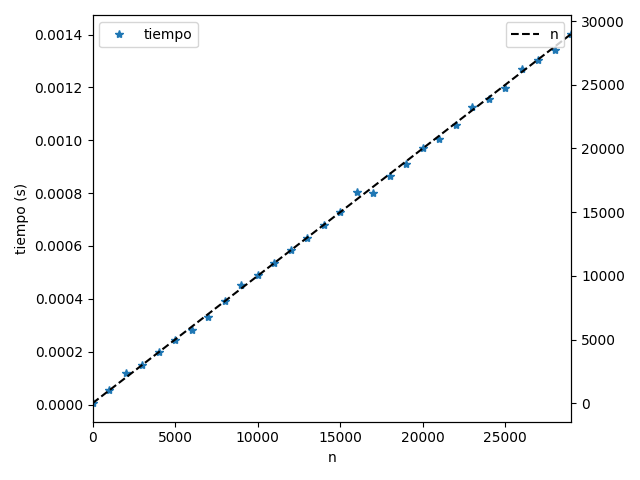
\includegraphics[scale=0.9]{revertirAudio.png}
\centering
\end{figure}  

\begin{figure}
\subsection*{limpiarAudio}
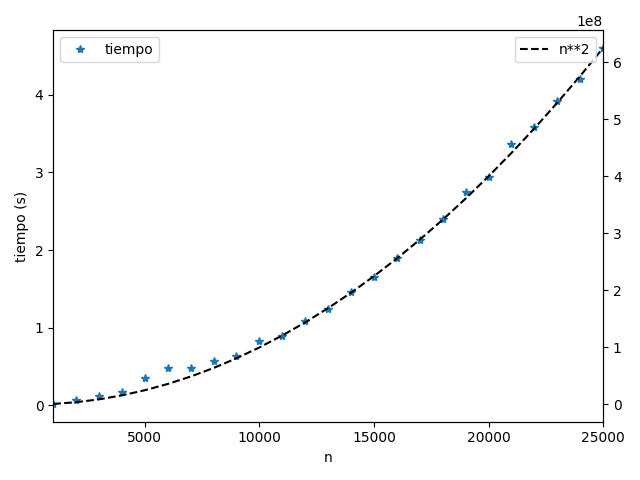
\includegraphics[scale=0.9]{limpiarAudio.png}
\centering
\end{figure} 








\end{document}












